\documentclass{beamer}
% \usepackage{animate}
\usepackage{multimedia}
\usepackage[english,russian]{babel}

\usepackage{pgfpages}
\setbeameroption{show notes on second screen}
%https://tug.ctan.org/macros/latex/contrib/beamer/doc/beameruserguide.pdf

\usepackage[T2A]{fontenc}
\usepackage[utf8]{inputenc}

\setbeamertemplate{caption}[numbered]

\usetheme{CambridgeUS}
\usecolortheme{dolphin}

\title[Сплайны]{Текстуры}
\author[Быковских Д.А.]{Быковских Дмитрий Александрович}
\date{16.11.2024}

\begin{document}
	\begin{frame}
		\titlepage
	% картинка с питером
	\end{frame}

	\begin{frame}{Содержание}
		Определение

		Наложение текстур

	\end{frame}

	\begin{frame}{Определение}
		Текстура (texture) --- массив данных (одномерный или многомерный).\\
		Элементом текстуры (texture element) является тексел (texel).\\
		
		При рендеринге 3D-объекта тексели из текстуры преобразуются в пиксели на экране.\\
		Например, текстура может содержать характеристики цвета (RGB).\\
				
		% Текстура описывает тактильные или визуальные характеристики поверхности, которые можно воспринимать через осязание или зрение. 
		% В контексте изображений или компьютерного зрения текстура определяет распределение интенсивности или цвета пикселей на изображении.\\


		%https://blender3d.com.ua/texel-density/

		\note{
			\begin{figure} 
				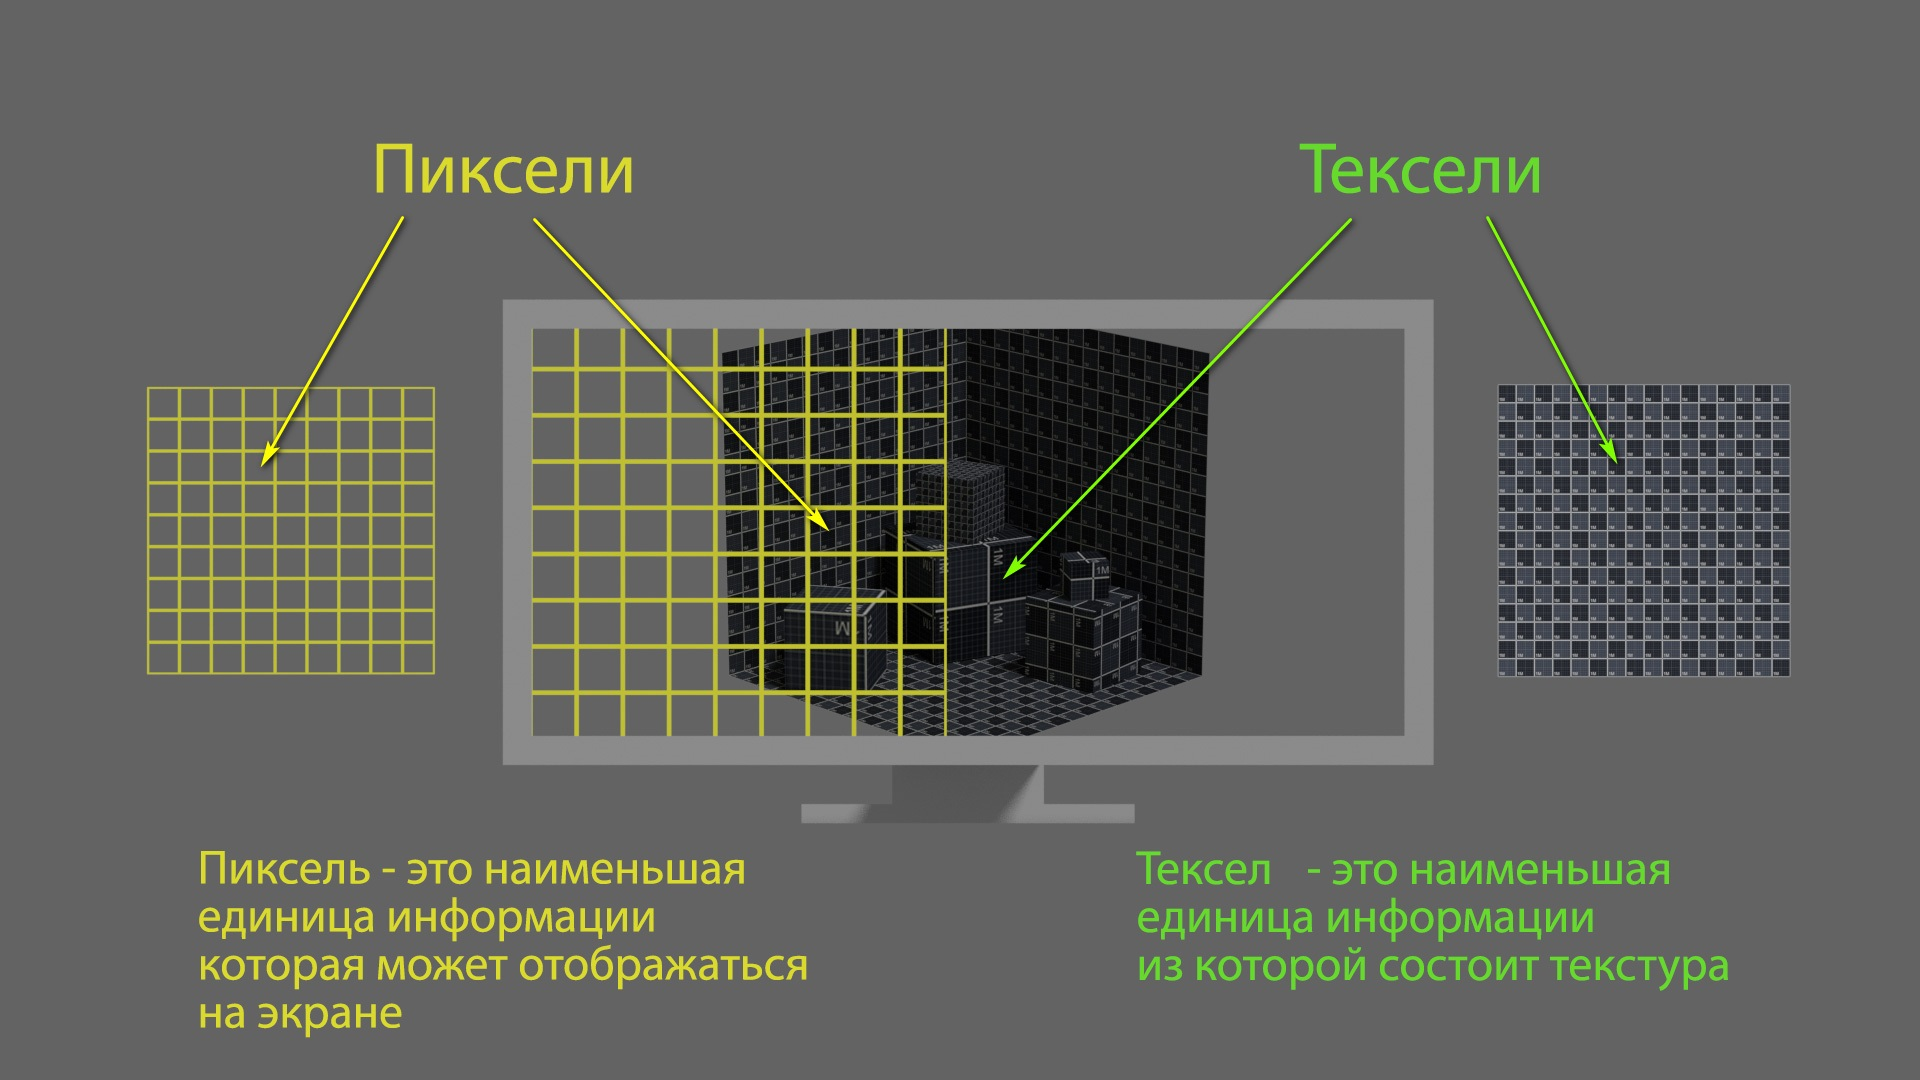
\includegraphics[width=0.9\textwidth]{images/texel.jpg}
				\caption{Процесс преобразования текселей в пиксели на экране}
			\end{figure}
		}
	\end{frame}

	\begin{frame}{Текстурное отображение (Texture Mapping)}

		Texture Mapping (текстурное отображение) --- процесс проецирования текстуры (2D-изображения) на поверхность 3D-объекта.  \\
		Этот процесс устанавливает связь между координатами объекта (в 3D-пространстве) и координатами текстуры (в 2D-пространстве) посредством определения соответствия участков текстуры для каждой точке поверхности объекта.\\

		В качестве дополнительного атрибута для каждой вершины объекта, имеющей координаты, указывается текстурные координаты (или UV-координаты).\\
		
		Примечание.\\
		Генерацию UV-развертки для объекта можно выполнить автоматически, например, с помощью редактора blender.\\


		\note{
			% https://kwojcicki.github.io/blog/NEAREST-NEIGHBOUR
			\begin{figure} 
				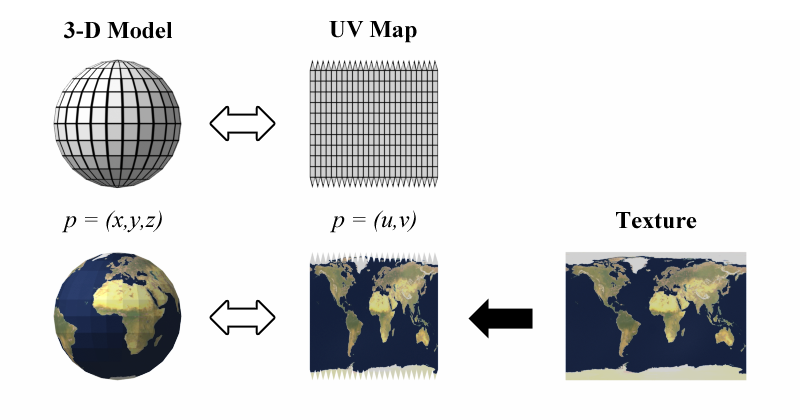
\includegraphics[width=1.0\textwidth]{images/UVMapping.png}
				\caption{uv-развертка (uv-mapping) }
			\end{figure}
		}
	\end{frame}
	
	\begin{frame}{Наложение текстур}
		Texture Sampling (сэмплирование) --- процесс извлечения данных из текстуры (например, цвета или других атрибутов) в заданной точке на основе интерполированных UV-координат, которые были рассчитаны автоматически на этапе растеризации.\\
		% Примечание.\\
		% Промежуточные значения UV-координат определяются автоматически.\\

		% \if 0
		% \begin{columns}
		% 	\begin{column}{0.5\textwidth}
		% 		ввв
		% 	\end{column}
		% 	\begin{column}{0.5\textwidth}
		% 		ываыа
		% 	\end{column}
		% \end{columns}
		% \fi


		\note{
			\begin{figure} 
				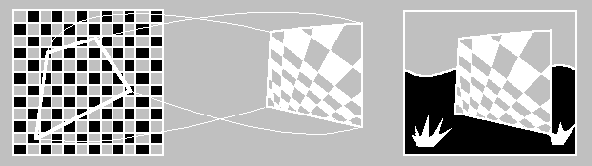
\includegraphics[width=\textwidth]{images/mapping.png}
				% 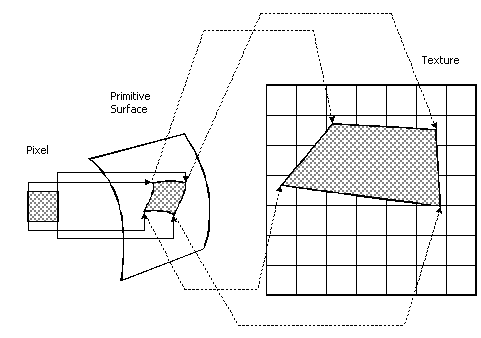
\includegraphics[width=0.4\textwidth]{images/texture_mapping.png}
				\scriptsize
				\begin{columns}
					\begin{column}{0.31\textwidth}
						Пространство текстуры \\
						% texture space
						Координаты текстур \\
						uv-space \\
					\end{column}
					\begin{column}{0.32\textwidth}
						Пространство объектов \\
						% object space
						Параметры поверхности \\
						xyz-space \\
					\end{column}
					\begin{column}{0.36\textwidth}
						Пространство изображения \\
						% screen space
						Координаты пикселей \\
						xy-space
					\end{column}
				\end{columns}
				\caption{Схема наложения текстуры на поверхность объекта}
			\end{figure}
			% https://learn.microsoft.com/en-us/windows/win32/direct3d9/texture-coordinates
		}
	\end{frame}

	\if 0
	\begin{frame}{Наложение текстур}

		\hfill Пространство текстуры \\
		% texture space
		\hfill (в нормализованном виде) \\
		\hfill Координаты текстур \\
		\hfill uv-space

		Преобразование поверхностной текстуры\\ (Texture Mapping)

		\hfill Пространство объектов \\
			% object space
		\hfill Параметры поверхности \\
		\hfill xyz-space
		
		Преобразование растеризация \\ (Texture Sampling)
		
		\hfill Пространство изображений \\
		% screen space
		\hfill Координаты пикселей \\
		\hfill xy-space
		
		\note{
			\begin{figure} 
				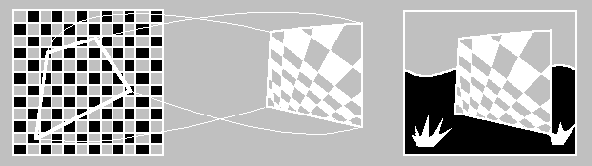
\includegraphics[width=\textwidth]{images/mapping.png}
				% 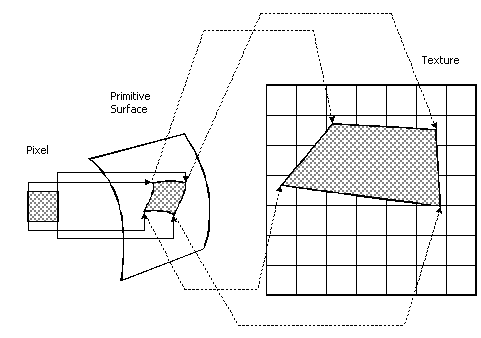
\includegraphics[width=0.4\textwidth]{images/texture_mapping.png}
				\caption{Пример текстуры}
			\end{figure}

			Примечание. \\
			направление наложения \\
			объект проецируется на текстуре

			Параметрическое преобразование
		}
		% https://learn.microsoft.com/en-us/windows/win32/direct3d9/texture-coordinates

	\end{frame}


	\begin{frame}{Пример (код)}
		%Термин происходит из математики и цифровой обработки сигналов, где он означает измерение значений сигнала в определённых точках.

		\begin{columns}
			\begin{column}{0.5\textwidth}
				% #version 330 core

				% layout(location = 0) in vec3 aPos;        // Позиция вершины
				% layout(location = 1) in vec2 aTexCoord;   // UV-координаты вершины

				% out vec2 TexCoord; // Передача UV-координат во фрагментный шейдер

				% uniform mat4 model;
				% uniform mat4 view;
				% uniform mat4 projection;

				% void main() {
				% 		// Преобразование позиции вершины в пространство экрана
				% 		gl_Position = projection * view * model * vec4(aPos, 1.0);
						
				% 		// Передача UV-координат во фрагментный шейдер
				% 		TexCoord = aTexCoord;
				% }
			\end{column}
			\begin{column}{0.5\textwidth}
				ываыа
			\end{column}
		\end{columns}

	\end{frame}
	\fi

	% \begin{frame}{GPU Pipeline}

	% 	Слайды с конвейером трехмерного преобразования
	% 	L1-Introduction и L2-Graphics\_pipeline.
	% 	% Vertex Shader \\
	% 	% Rasterizer \\
	% 	% Fragment Shader and Texture Unit \\
	% 	% Image

	% 	% \note{
	% 	% 	\begin{figure} 
	% 	% 		\includegraphics[width=0.9\textwidth]{images/}
	% 	% 		\caption{Пример текстуры}
	% 	% 	\end{figure}
	% 	% }
	% \end{frame}

	\begin{frame}{Эффект ступенчатости}{Aliasing}
		Термин "aliasing" (ступенчатость) происходит от слова "alias"\ в английском языке, которое означает "псевдоним"\ или "иное имя". 
		
		{\footnotesize
		В компьютерной графике, ступенчатость возникает, когда высокочастотные детали изображения (например, тонкие линии или края) не могут быть правильно представлены на низкочастотной сетке пикселей. 
		Это приводит к появлению артефактов в виде ступенчатости или "псевдонимов"\ вдоль краев объектов. 
		%Антиалиасинг, как техника, направленная на уменьшение этих ступенчатых эффектов, призвана устранять или смягчать эти "псевдонимы" на изображениях, делая их более гладкими и природными визуально.
		}
		
		Antialiasing (сглаживание) --- техника в компьютерной графике, направленная на уменьшение ступенчатости (или зубчатости) на изображениях, особенно заметной на краях объектов или диагоналях. 
				
		{\footnotesize
		Ступенчатость возникает из-за ограниченного числа пикселей, используемых для представления изображения, что может создавать впечатление неровных и недостаточно гладких линий.
		Антиалиасинг достигается путем размытия переходов между цветами на краях объектов. Это может быть выполнено различными методами, включая сглаживание, суперсэмплирование и другие. %Результатом является более гладкое и естественное визуальное восприятие изображения.
		}
		\note{
			% https://www.pcmag.com/encyclopedia/term/anti-aliasing
			\begin{figure} 
				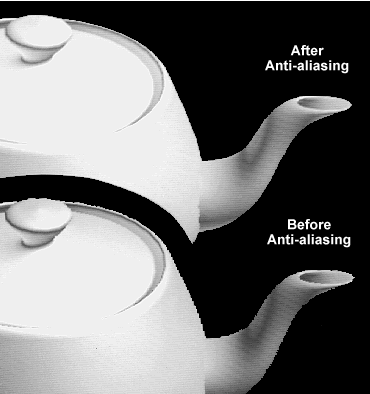
\includegraphics[width=0.5\textwidth]{images/anti-aliasing.png}
				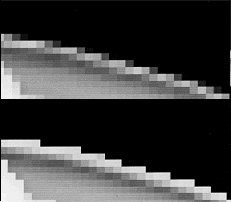
\includegraphics[width=0.45\textwidth]{images/anti-aliasing_extra.png}
				\caption{Пример эффекта ступенчатости}
			\end{figure}
		}

	\end{frame}

	\begin{frame}{Способы наложения текстур}

		
		% Sampling (выборка) --- процесс извлечения данных из дискретного пространства, например, из текстуры.

		\begin{enumerate}
			\item Метод ближайшего соседа (Nearest-Neighbour Method) (без фильтрации)
			\item билинейная фильтрация (Bilinear Filtering)
			\item бикубическая фильтрация 
			\item трилинейная фильтрация (Trilinear Filtering)
			\item анизотропная фильтрация (Anisotropic Filtering)
		\end{enumerate}

		Примечание. \\ 
		Используется аппаратно-программная поддержка.\\


		% \note{
		% 	% https://kwojcicki.github.io/blog/NEAREST-NEIGHBOUR
		% 	\begin{figure} 
		% 		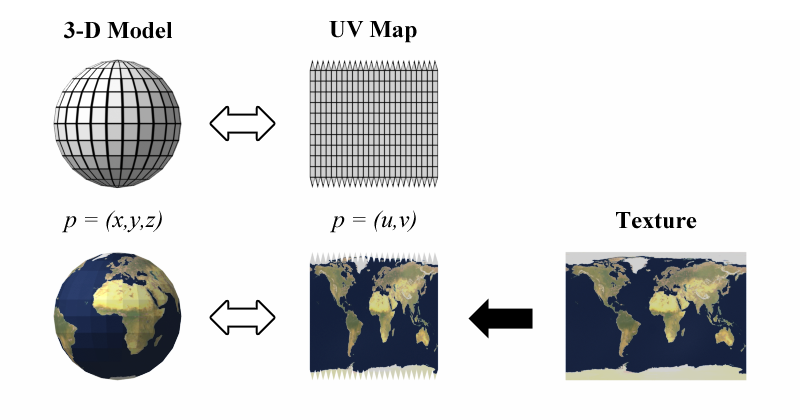
\includegraphics[width=0.8\textwidth]{images/UVMapping.png}
		% 		\caption{uv-развертка (uv-mapping) }
		% 	\end{figure}
		% }
	\end{frame}

	\begin{frame}{Метод ближайшего соседа}{Nearest-Neighbour Method}

	 	Метод ближайшего соседа --- основан на ступенчатой интерполяции.

		Этот метод использует значения самого близкого пикселя для вычисления нового значения после масштабирования.

		Когда изображение масштабируется в больший размер, каждый новый пиксель получает значение из ближайшего пикселя в оригинальном изображении. Аналогично, при уменьшении размера каждый новый пиксель получает значение из ближайшего пикселя, что может быть менее точным представлением данных.
				
		Вот примеры использования:
		
		\begin{enumerate}
			% \item 
			% Бинарные изображения (черно-белые; только два цвета).
			\item 
			Приложения с низкими требованиями к производительности.
		\end{enumerate}




		% методом ближайшего соседа (ступенчатая интерполяция) —
		% $P_1; P_2; P_3$
		% качество
		% Nearest Texel for current Pixel
		% example
		% $u = \alpha u_0 + \beta u_1 + \gamma u_2$
		\note{
			% https://kwojcicki.github.io/blog/NEAREST-NEIGHBOUR
			\begin{figure} 
				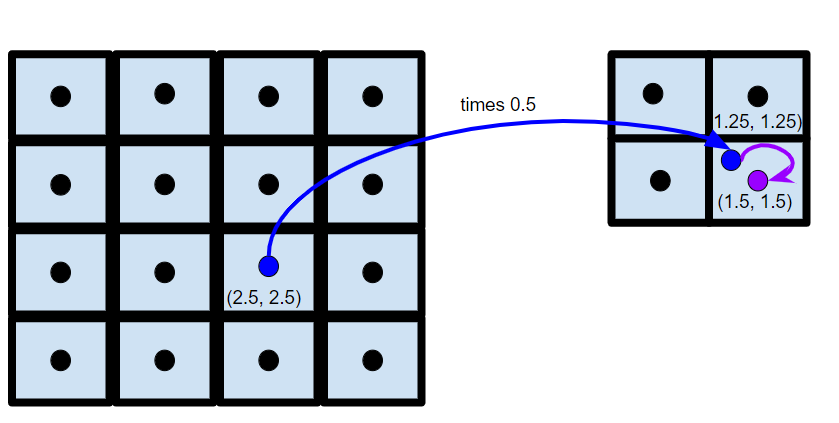
\includegraphics[width=0.8\textwidth]{images/nn_filtering.png}
				\caption{Пример текстуры}
			\end{figure}
		}

		% https://community.adobe.com/t5/substance-3d-painter-discussions/viewport-texturing-filtering/td-p/13444697
		
	\end{frame}
	
	\begin{frame}{Текстурная фильтрация}{Texture Filtering}
		Фильтрации основаны на интерполяции
		% Interpolation
		
		% Bilinear Filtering
		Билинейная фильтрация --- метод фильтрации текстур в компьютерной графике, используемый для улучшения качества отображения текстур при масштабировании. Этот метод предназначен для устранения ступенчатости и артефактов, которые могут возникнуть при изменении размера текстур.


		% Bicubic Filtering
		Бикубическая фильтрация --- метод фильтрации, используемый в компьютерной графике, который обеспечивает более точное и качественное увеличение изображений и текстур по сравнению с билинейной фильтрацией. Этот метод часто применяется при изменении размера изображений.

		{\footnotesize
			Основная идея бикубической фильтрации заключается в том, чтобы использовать значения не только ближайших пикселей, как в билинейной фильтрации, но и значения соседних пикселей, чтобы создать более гладкие и точные результаты. Алгоритм использует кубические полиномы для интерполяции значений пикселей.
		}

		% Слайды с конвейером трехмерного преобразования
		% L1-Introduction и L5-Graphics\_pipeline.

		\note{
			\begin{figure} 
				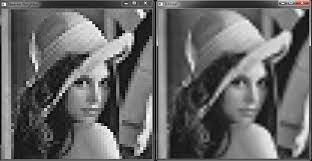
\includegraphics[width=\textwidth]{images/bilinear_filtering.jpg}
				\caption{Сравнение фильтраций: метод ближайшего соседа (слева) и билинейная фильтрация (справа)}
			\end{figure}
		}

	\end{frame}

	\begin{frame}{Mip-текстура}{Mipmaps}
		
		Mipmap (Multum In Parvo, т.е. многое в малом) представляет собой предварительно созданный набор изображений с разными разрешениями исходной текстуры. Каждое последующее изображение в этом наборе имеет размер в половину (или в другой пропорции) меньший, чем предыдущее. Таким образом, создается иерархия текстур, где каждый уровень представляет собой изображение с определенным уровнем детализации.

		Использование такой текстуры позволяет избежать артефактов, таких как мерцание и дрожание текстур на дальних объектах, и в то же время повысить производительность при рендеринге.
		% 		MIP-mapping увеличивает расход видеопамяти на треть:
		% 	\[
		% 		\sum_{i=0}^\infty \left( \frac {1} {4} \right)^i = 1 \frac {1} {3}
		% 	\]

		% При наложении текстур вычисляется расстояние до объекта и номер текстуры находится по формуле:
		% \[
		% 	{mip\_level} = \log_2 \left( \frac {{distance}} {{texel\_size} \cdot {camera\_resolution}} \right) + {mip\_bias}
		% 	,
		% 	\]
		% 	$mip\_bias$ --- число, позволяющее выбирать более или менее детальную текстуру, чем даёт формула.
		% где $resolution$ --- разрешение виртуальной камеры (количество пикселей, которое будет в объекте размером в 1 ед., расположенном в 1 ед. от камеры), $texelsize$ --- размер текселя в единицах трёхмерного мира, $dist$ --- расстояние до объекта в тех же единицах, 
		% Это число округляется до целого, и текстура с соответствующим номером (нулевая — самая детальная, первая — вдвое меньшая и т. д.) накладывается на объект.

		\note{
			\begin{figure} 
				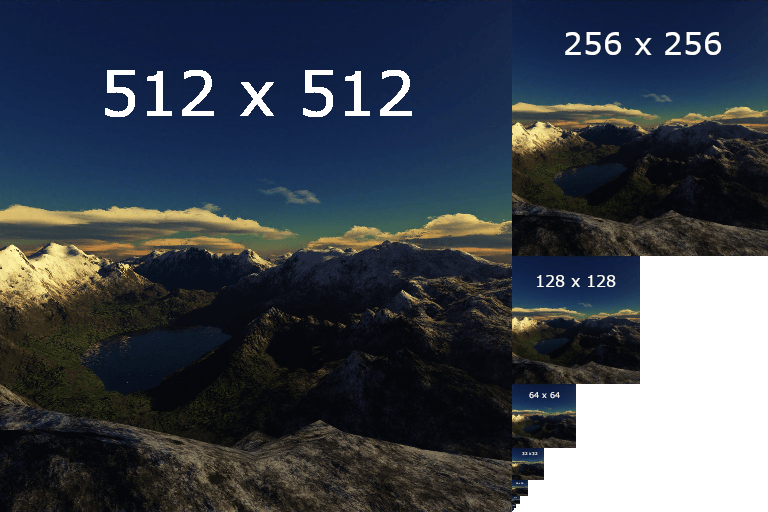
\includegraphics[width=0.75\textwidth]{images/mipmap.png}
				\caption{Mip-текстура}
			\end{figure}
		}

	\end{frame}

	\begin{frame}{Трилинейная фильтрация}{Trilinear Filter}
		Трилинейная фильтрация --- техника фильтрации текстур в компьютерной графике, предназначенная для улучшения качества отображения при масштабировании текстур на различных расстояниях и углах обзора.

		Трилинейная фильтрация включает в себя два этапа фильтрации:
		\begin{enumerate}
			\item 
			Mipmap фильтрация. Выбор подходящего уровня mipmap в зависимости от расстояния до объекта.
			\item
			Билинейная фильтрация. Интерполяция значений внутри выбранного уровня mipmap.
		\end{enumerate}


		Трилинейная фильтрация обеспечивает более гладкое и качественное отображение текстур, особенно при масштабировании, так как она учитывает как изменения масштаба, так и углы обзора.

		Недостаток такой техники заключается в том, что все цвета вдалеке сильно смешиваются.

		\note{
			\begin{figure} 
				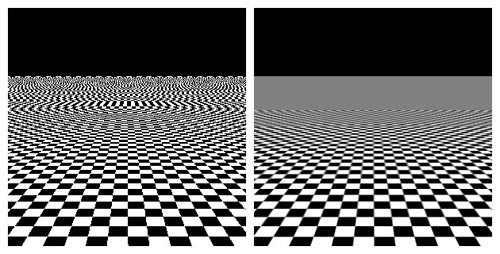
\includegraphics[width=\textwidth]{images/bi_tri_linear_filtering.jpg}
				\caption{Сравнение методов фильтрации: билинейной (слева) и трилинейной (справа)}
			\end{figure}
		}

	\end{frame}


	
	
	\begin{frame}{Анизатропная фильтрация}{Anisotropic Filtering (with Mipmaps)}


		
		Анизотропная фильтрация --- техника в компьютерной графике, применяемая к текстурам для улучшения качества отображения при различных углах обзора. Эта техника особенно полезна при работе с текстурами, которые наклонены под разными углами или отображаются под разными ракурсами.
		
		Фактически убирает размытие при смешивании за счет того, что работает в трех измерениях.
		
		% Преимущества анизотропной фильтрации включают:
		
		% 		Качество отображения: Улучшение качества текстур при различных углах обзора, что особенно важно для текстур, ориентированных под углом к камере.
		
		% 		Плавные переходы: Снижение артефактов, таких как ступенчатость, и обеспечение более плавных переходов между пикселями текстуры.
		
		% 		Более точное отображение деталей: Анизотропная фильтрация позволяет более точно отобразить детали текстур, особенно при масштабировании.
		
		% Однако использование анизотропной фильтрации может быть более ресурсоемким процессом по сравнению с обычной билинейной фильтрацией, поэтому ее применяют там, где требуется более высокое качество отображения.
	
		\note{
			\begin{figure} 
				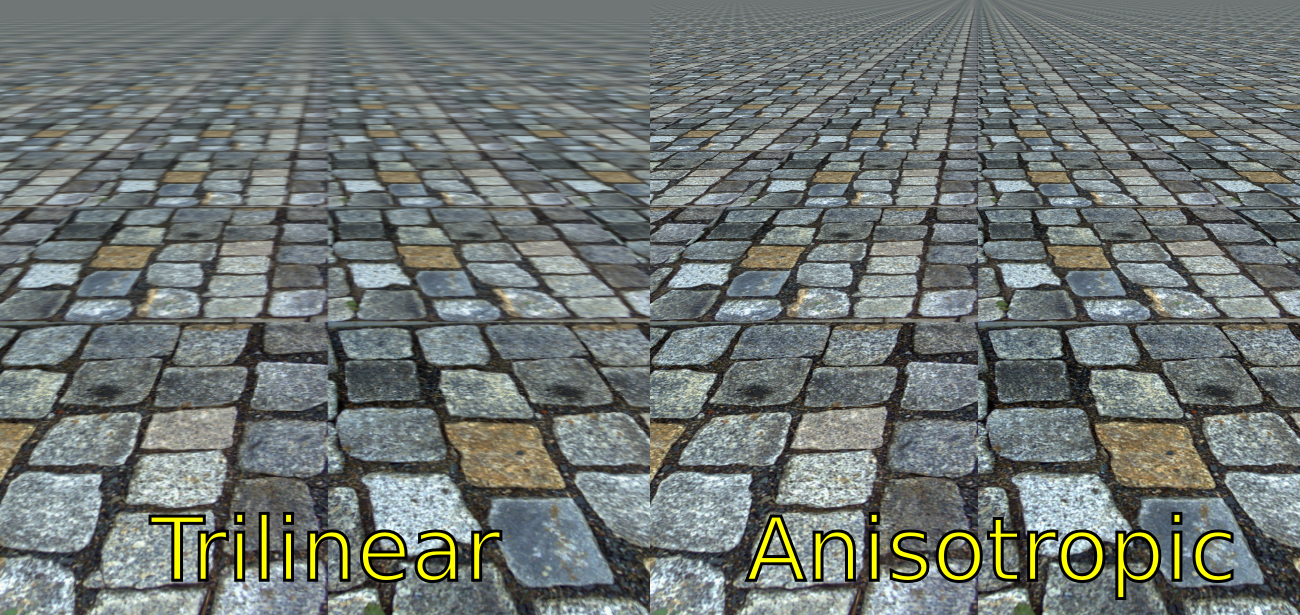
\includegraphics[width=\textwidth]{images/anisotropic_filtering.png}
				\caption{Сравнение методов фильтрации: трилинейной (слева) и анизатропной (справа)}
			\end{figure}
		}


	\end{frame}


	\begin{frame}{Классификация}

		Основные виды
		\begin{enumerate}
			\item Исходные изображения;
			\item MIP-текстуры;
			\item Процедурные текстуры. %Procedural Textures c=f(u) флаги
			%working set попадают в текстурную память
		\end{enumerate}
		
		Специализированные
		\begin{enumerate}
			\item Карта нормалей (Normal Map);
			\item Карта высот (Height Map);
			
			\item Карта окклюзии (Ambient Occlusion Map);
			\item Карта тени (Shadow Map);
		
			\item Карта смешивания (Blend Map);
		\end{enumerate}

		\note{
			Эффект наложения текстур на полигональные модели привел к большому прорыву. 
			\\До сих пор использование текстур является основой для построения реалистичного изображения. %Количество видов поражает!
		}
	\end{frame}

	\begin{frame}{Процедурные текстуры}

		Процедурные текстуры --- текстуры, которые генерируются алгоритмически, а не создаются вручную или с помощью изображений. 
		Они используют математические функции и алгоритмы для создания деталей, шумов, узоров и других характеристик текстуры. Этот подход позволяет создавать бесконечные и вариативные текстуры, которые могут быть адаптированы под различные условия и среды.

Примеры процедурных текстур:
\begin{enumerate}
	\item 
	Шум Перлина (Perlin Noise)%: Это один из наиболее распространенных алгоритмов для генерации текстурного шума, используемого в компьютерной графике и компьютерной генерации изображений. Он может быть использован для создания реалистичных поверхностей, таких как горы, облака, вода и др.
	\item
	Фрактальные текстуры%: Алгоритмы фрактальной генерации могут быть использованы для создания текстур с самоподобными деталями на различных уровнях масштаба. Это может быть полезно для создания разнообразных природных элементов, таких как леса, горы и т. д.
	\item
	Текстуры шероховатости%: Процедурные алгоритмы могут быть использованы для создания текстур с различными уровнями шероховатости, что может быть полезно для реализации реалистичных материалов, таких как камень, дерево и т. д.
	\item
	Марблинг и деревообразные текстуры%: Процедурные текстуры могут эмулировать множество различных природных и искусственных материалов, таких как мрамор, дерево, металл и другие.
\end{enumerate}

	Преимущество процедурных текстур заключается в их гибкости, возможности легкой настройки и создания уникальных вариантов текстур без необходимости хранения больших файлов изображений.

		\note{
			% http://www.upvector.com/?section=Tutorials&subsection=Intro%20to%20Procedural%20Textures
				\begin{figure} 
					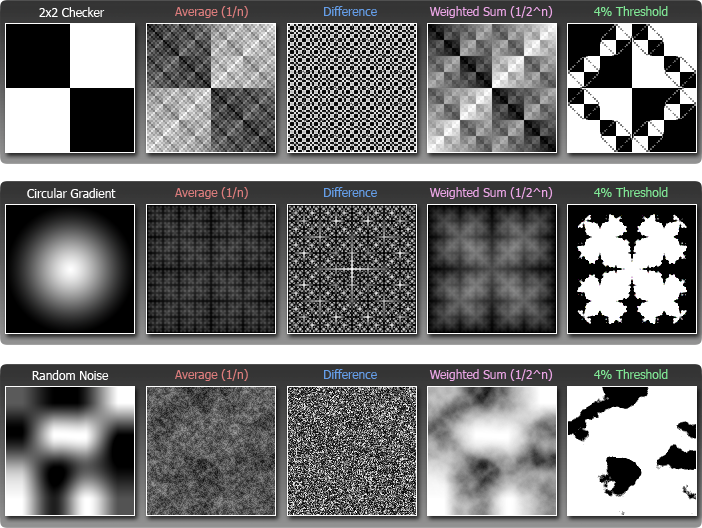
\includegraphics[width=0.7\textwidth]{images/procedural_textures.png}
					\caption{Процедурные текстуры}
				\end{figure}
		}
	\end{frame}


	\begin{frame}{Специализированные текстуры}
		\begin{enumerate}
			\item Карта нормалей (Normal Map) \\
			Используется для добавления деталей к поверхности объекта, не увеличивая количество полигонов. 
			Цвет каждого пикселя карты нормалей представляет собой вектор, указывающий направление нормали к поверхности в данной точке.
			% https://ycpcs.github.io/cs470-fall2014/labs/lab12-2.html
			\item Карта высот (Height Map) \\
			Используется для создания рельефности поверхности. 
			Значения яркости пикселей определяют высоту соответствующих точек на поверхности объекта.
			%\item Карта выпуклостей (Bump map): используется для создания иллюзии высоких и низких точек на поверхности, но без фактического изменения геометрии. Он воздействует на освещение, создавая тени и подчеркивая детали, но не изменяет форму самого объекта.
	
		\end{enumerate}

		\footnotesize
		Этапы запекания (baking) текстур \\
		\begin{enumerate}
			\item 
			Создание из исходной (высокополигональной) модели низкополигональную модель путем отбрасывания вершин, сохраняя общие очертания модели.
			\item 
			Создание uv-развертки для низкополигональной модели.
			\item 
			Выбор тип карты для запекания и создание текстуры, куда будет сохранять результат.
			\item 
			Выполнить запекание, указав нужные параметры.
		\end{enumerate}


		
		\note{
			{
			\footnotesize
			Примечание.
			Позволяет сохранить высокую детализацию, минимизируя вычислительные затраты
			}
			% https://typhen.artstation.com/blog/BDr6/this-is-normal-2-baking-normal-maps
			\begin{figure} 
				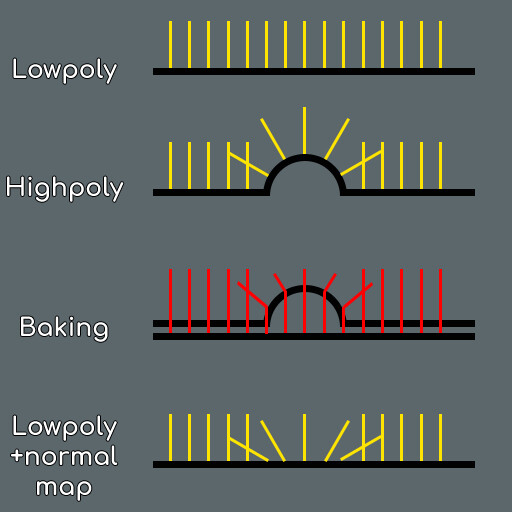
\includegraphics[width=0.45\textwidth]{images/Baking.jpg}
				\caption{Схема процесса запекания текстуры}
			\end{figure}

		}
	\end{frame}

	\begin{frame}{Специализированные текстуры}{связанные с тенями}
		\begin{enumerate}
			\item Карта окружающего затенения (Ambient Occlusion Map)\\ 
			Описывает, насколько освещен каждый пиксель, учитывая его окружение. Темные области могут указывать на близость объектов или узкие пространства, где освещение ограничено.
			\item Карта теней (Shadow Map)\\ 
			Используется для определения областей, находящихся в тени.
		\end{enumerate}
		
		Примечание.\\
		Текстура, в которой хранятся тени от рассеянного света, содержит оттенки серого.\\
		Подходит для сцены с неподвижными источниками света.\\
		Разделение необходимо в случаи изменения степени освещенности сцены. \\
	
			\note{
				% https://3dclub.com/blog/kak-ispolzovat-karty-ao
				% https://gamedev.ru/code/forum/?id=175200
				\begin{figure} 
					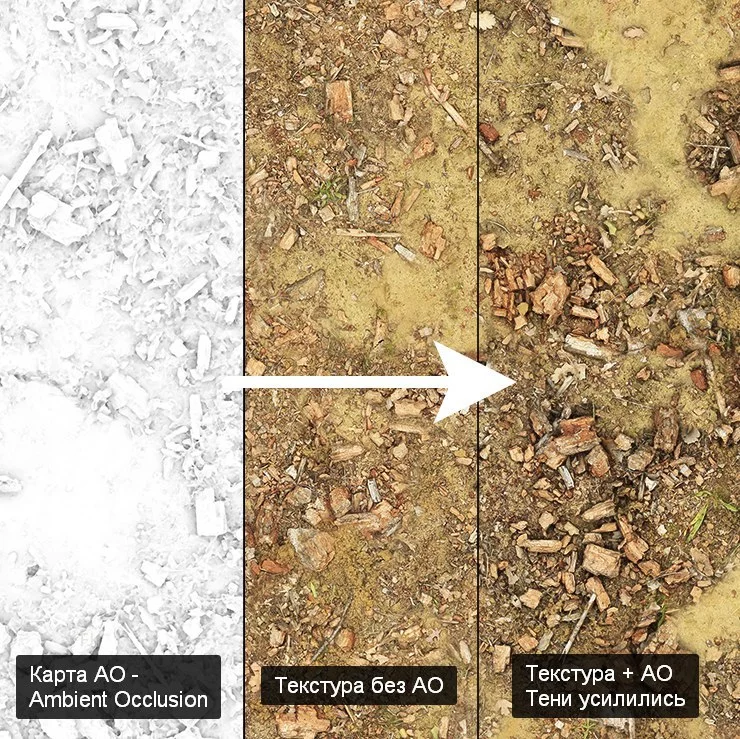
\includegraphics[width=0.45\textwidth]{images/ambient_occlusion.png}
					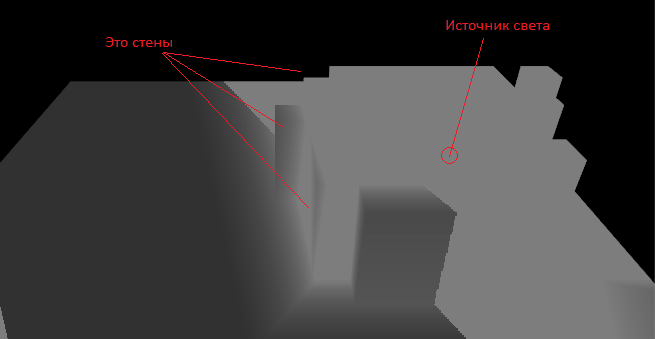
\includegraphics[width=0.5\textwidth]{images/shadow_mapping.png}
					\caption{Специализированные текстуры: Карта окружающего затенения (слева) и карта теней (справа)}
				\end{figure}
			}
	\end{frame}

	\begin{frame}{Специализированные текстуры}
		\begin{enumerate}		
			\item Карта смешивания (Blend Map)\\
			Применяется для смешивания нескольких текстур в зависимости от определенных условий. Например, можно использовать карту смешивания для определения, где на объекте применять текстуру травы, а где текстуру камня.
			\end{enumerate}

			\begin{figure} 
				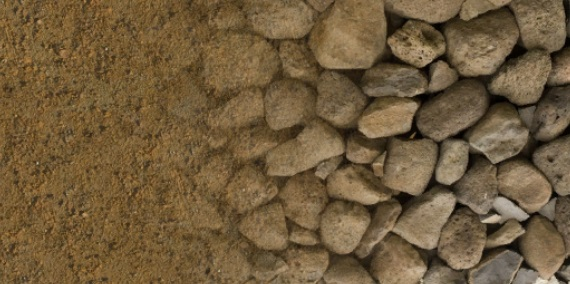
\includegraphics[width=0.5\textwidth]{images/blend_1.jpg}
				\caption{Проблема при смешивании}
			\end{figure}

			% https://habr.com/ru/articles/180743/
			\note{
				\begin{figure}
					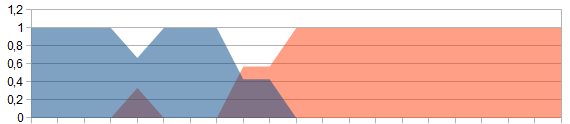
\includegraphics[width=0.7\textwidth]{images/blend_4.png}
					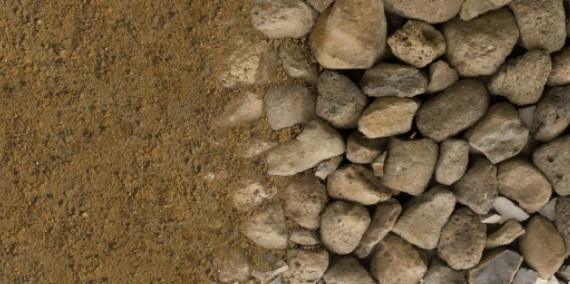
\includegraphics[width=0.7\textwidth]{images/blend_3.jpg}
					\caption{Карта смешивания и результат}
				\end{figure}
	
			}

	\end{frame}

	\begin{frame}{Заключение}
		Литература
		\begin{enumerate}
			\item \href{http://www.upvector.com/?section=Tutorials&subsection=Intro\ to\ Procedural\ Textures}{Procedural Textures}
			\item \href{http://euklid.mi.uni-koeln.de/c/mirror/www.cs.curtin.edu.au/units/cg351-551/notes/lect9i1.html}{Displaying Textures on the Screen}
			\item \href{https://learn.microsoft.com/en-us/windows/win32/direct3d9/texture-coordinates}{Texture Coordinates}
			\item \href{https://www.pcmag.com/encyclopedia/term/anti-aliasing}{Anti-Aliasing}
			\item \href{https://kwojcicki.github.io/blog/NEAREST-NEIGHBOUR}{Nearest Neighbour Interpolation}
			\item \href{https://community.adobe.com/t5/substance-3d-painter-discussions/viewport-texturing-filtering/td-p/13444697}{Viewport Texturing Filtering}
			% \item \href{http://www.upvector.com/?section=Tutorials&subsection=Intro to Procedural\ Textures}{text}
			\item \href{https://ycpcs.github.io/cs470-fall2014/labs/lab12-2.html}{Normal and Displacement Mapping}
			\item \href{https://typhen.artstation.com/blog/BDr6/this-is-normal-2-baking-normal-maps}{Baking Normal Maps}
			\item \href{https://3dclub.com/blog/kak-ispolzovat-karty-ao}{Что такое Ambient Occlusion}
			\item \href{https://gamedev.ru/code/forum/?id=175200}{Shadow Mapping}
			\item \href{https://habr.com/ru/articles/180743}{Смешивание текстур ландшафта}
		\end{enumerate}

	\end{frame}

	\end{document}